% THIS TEMPLATE IS A WORK IN PROGRESS
% Adapted from an original template by faculty at Reykjavik University, Iceland

\documentclass{scrartcl}
\input{File_Setup.tex}
\usepackage{graphicx,epsfig}
\usepackage{algorithm}
\usepackage{algpseudocode}
\usepackage{listings}
\usepackage{xcolor}
\hypersetup{
   colorlinks   = true,                               %Colours links instead of ugly boxes
   urlcolor     = blue,                               %Colour for external hyper links
   linkcolor    = blue,                               %Colour of internal links
   citecolor    = red,                                %Colour of citations
   setpagesize  = false,
   linktocpage  = true,
}
\graphicspath{ {fig/} }

% Code listing style
\lstset{
    language=Python,
    basicstyle=\ttfamily\small,
    keywordstyle=\color{blue},
    commentstyle=\color{green!60!black},
    stringstyle=\color{orange},
    showstringspaces=false,
    breaklines=true,
    frame=single,
    numbers=left,
    numberstyle=\tiny\color{gray}
}

\renewenvironment{abstract}{
    \centering
    \textbf{Abstract}
    \vspace{0.5cm}
    \par\itshape
    \begin{samepage}
}{\end{samepage}
    \noindent\ignorespaces
}
% ------------------------------------------------------------------------------------------------------------------------

\begin{document}
%Title of the report, name of coworkers and dates (of experiment and of report).
\begin{titlepage}
	\centering
	
\includegraphics[width=0.6\textwidth]{fig/GW_logo-eps-converted-to.pdf}\par
	\vspace{2cm}
	%%%% COMMENT OUT irrelevant lines below: Data Science OR Computer Science OR none
	{\scshape\LARGE Data Science Program \par}
	{\scshape\Large Capstone Report - Fall 2025\par}
	%{\large \today\par}
	\vspace{1cm}
	%%%% PROJECT TITLE
	{\huge\bfseries Reinforcement Learning for Pseudo-Labeling in Semi-Supervised Learning\par}
	\vspace{1.5cm}
	%%%% AUTHOR(S)
	{\Large\itshape Aishwarya Maddula, Deepika Reddygari\\}\par
  {\Large\itshape Prudhvi Chekuri, Phanindra Kalaga\\}\par
	\vspace{1.5cm}
	supervised by\par
	%%%% SUPERVISOR(S)
	Prof. Tyler Wallett\\
	Dr. Amir Jafari

	\vfill
	\begin{abstract}
	    Semi-supervised learning leverages abundant unlabeled data to improve performance when labeled data is scarce. This project develops a reinforcement learning (RL) framework for intelligent pseudo-labeling, where an RL agent learns to assign high-quality pseudo-labels to unlabeled samples. We implement and evaluate a Policy Gradient approach on MNIST and a Reinforcement Learning-Guided Semi-Supervised Learning (RLGSSL) method inspired by recent research. Our results demonstrate that confidence-based rewards and adaptive training can improve pseudo-labeling quality, though challenges remain in computational complexity and reward design. These findings provide insights for future work in RL-guided semi-supervised learning.
	\end{abstract}
	\vfill
% Bottom of the page
\end{titlepage}
\tableofcontents
\newpage
% ------------------------------------------------------------------------------------------------------------------------


\section{Introduction}

In modern machine learning applications, obtaining large quantities of labeled training data is often expensive, time-consuming, and requires domain expertise. Semi-supervised learning (SSL) offers a promising solution by leveraging both limited labeled data and abundant unlabeled data to improve model performance. A key technique in SSL is pseudo-labeling, where a model assigns estimated labels to unlabeled samples, which are then used for further training.

Traditional pseudo-labeling approaches rely on simple heuristics such as confidence thresholds, often selecting pseudo-labels based solely on prediction confidence. However, these methods can propagate errors when incorrect high-confidence predictions are blindly accepted, leading to confirmation bias and degraded model performance.

This project addresses these limitations by framing pseudo-labeling as a reinforcement learning problem. By treating the selection and assignment of pseudo-labels as a sequential decision-making task, we enable an intelligent agent to learn optimal labeling strategies that balance exploration (diverse samples) and exploitation (high-confidence samples). 

\subsection{Project Objectives}

The primary objectives of this capstone project are:
\begin{enumerate}
    \item \textbf{RL Framework Development}: Design and implement a reinforcement learning framework that can automatically assign pseudo-labels to unlabeled data in a principled manner.
    \item \textbf{Custom Environment Design}: Build a custom OpenAI Gymnasium environment specifically tailored for the pseudo-labeling task, with carefully designed state spaces, action spaces, and reward functions.
    \item \textbf{Policy Gradient Implementation}: Implement and evaluate Policy Gradient methods (Actor-Critic) for learning pseudo-labeling strategies.
    \item \textbf{RLGSSL Exploration}: Investigate and implement the Reinforcement Learning-Guided Semi-Supervised Learning approach proposed by Heidari et al.~\cite{heidari2024rlgssl}, which integrates RL with teacher-student frameworks and mixup augmentation.
    \item \textbf{Empirical Evaluation}: Conduct comprehensive experiments on standard datasets (MNIST, CIFAR-10) to evaluate the effectiveness of RL-based pseudo-labeling approaches.
\end{enumerate}

\subsection{Project Scope}

This project explores two complementary approaches to RL-based pseudo-labeling:

\textbf{Approach 1: Custom RL Environment with Policy Gradients} -- We developed a complete RL framework from scratch, including:

\begin{figure}[H]
    \centering
    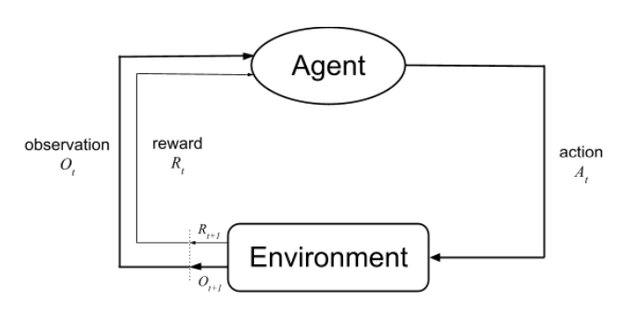
\includegraphics[width=0.8\textwidth]{fig/RL-agent-environment-loop.jpg}
    \caption{RL agent-environment loop. The agent selects actions and the environment responds and presents new observations and rewards to the agent again. The aim is for the agent to learn to maximize rewards through repeated interaction.}
    \label{fig:rl_agent_env_loop}
\end{figure}

\begin{itemize}
    \item A custom PseudoLabelEnv environment implementing the OpenAI Gymnasium interface.
    \item A state representation designed to capture both image features and model uncertainty.
    \item A discrete action space allowing the agent to assign pseudo-labels or defer judgment (skip).
    \item A confidence-driven reward structure to encourage high-quality labeling.
\end{itemize}



\textbf{Approach 2: RLGSSL Framework} -- Building on recent research, we investigated the RLGSSL approach which integrates:

\begin{figure}[H]
    \centering
    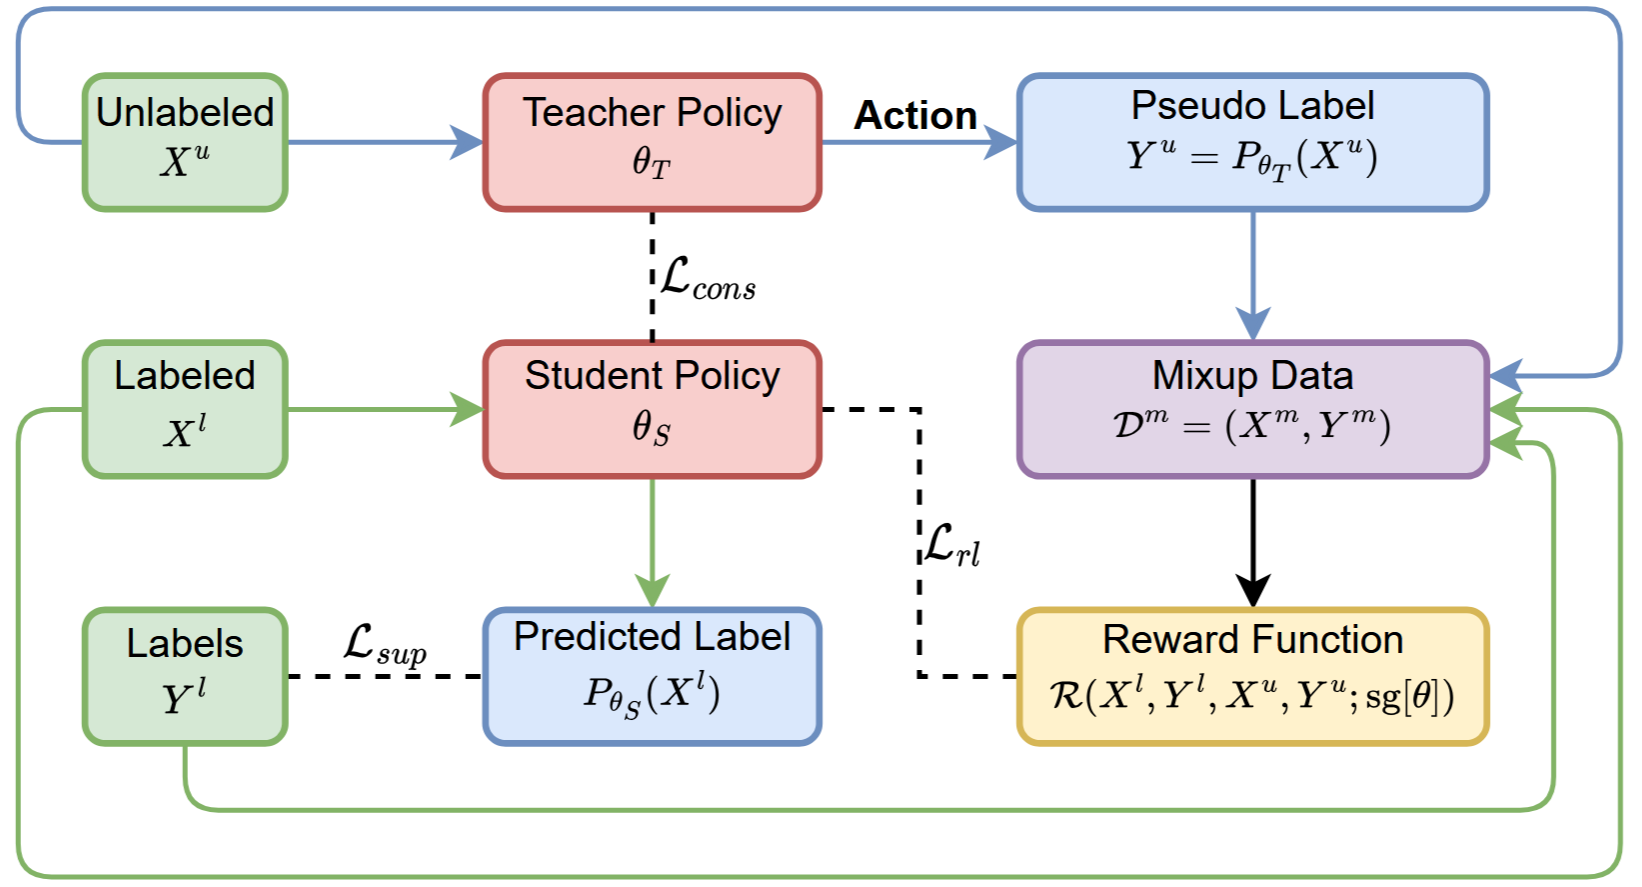
\includegraphics[width=0.8\textwidth]{fig/RLGSSL.png}
    \caption{Overview of the RLGSSL Framework. The prediction networks $(\theta_S,\, \theta_T)$ serve as the policy functions, and pseudo-labeling $(P_{\theta_T}(X^u))$ acts as the actions. The model has three loss terms in total: RL loss $(\mathcal{L}_{\mathrm{rl}})$, supervised loss $(\mathcal{L}_{\mathrm{sup}})$, and consistency loss $(\mathcal{L}_{\mathrm{cons}})$. The teacher policy function is used to execute the actions and compute the consistency loss, while the student policy function is used for all other aspects.}
    \label{fig:rl_agent_env_loop}
\end{figure}

\begin{itemize}
    \item A Teacher-Student framework utilizing Exponential Moving Average (EMA) for stable target generation.
    \item Mixup data augmentation to create a continuous training signal.
    \item A reinforcement learning reward signal derived from performance on synthetic mixup samples.
    \item Adaptive enhancements to the loss function to improve stability and diversity.
\end{itemize}

This report details our implementation methodology, experimental setup, results, challenges encountered, and insights gained throughout this capstone project.

% ------------------------------------------------------------------------------------------------------------------------
\section{Problem Statement}

\subsection{Semi-Supervised Learning Challenges}

Semi-supervised learning aims to leverage unlabeled data to improve model performance when labeled data is scarce. While pseudo-labeling has shown promise as a simple yet effective SSL technique, several fundamental challenges remain. The first is \textbf{confirmation bias}: traditional pseudo-labeling methods tend to reinforce existing model biases. When a model makes confident but incorrect predictions, using these as pseudo-labels amplifies errors through a feedback loop. The second is the \textbf{quality vs. quantity trade-off}: aggressive pseudo-labeling using low confidence thresholds provides more training data but risks adding noisy labels, while conservative approaches using high confidence thresholds ensure quality but fail to leverage the full potential of unlabeled data. Another challenge is \textbf{static decision rules}: existing methods typically use fixed heuristics (e.g., “accept if confidence $> 0.95$”) that do not adapt to the evolving model capabilities or dataset characteristics during training. Finally, the \textbf{sample selection strategy} is non-trivial, as determining which unlabeled samples should be pseudo-labeled at each training iteration requires balancing prediction confidence, sample diversity, and potential impact on model improvement.

\subsection{Reinforcement Learning Formulation}

To address these challenges, we formulate pseudo-labeling as a sequential decision-making problem suitable for reinforcement learning. This formulation enables \textbf{adaptive strategies}, where the RL agent learns to adjust its pseudo-labeling behavior based on accumulated experience and model evolution, as well as \textbf{exploration-exploitation balance}, where the agent naturally balances exploring uncertain samples versus exploiting high-confidence predictions.

\subsection{Technical Challenges}

Applying reinforcement learning to pseudo-labeling introduces several technical challenges. One is \textbf{state space design}, which involves determining effective feature representations that capture both image characteristics and model uncertainty. Another is \textbf{reward function engineering}, which requires designing reward signals that encourage correct pseudo-labeling while avoiding reward hacking and maintaining training stability. \textbf{Computational complexity} is also a major issue, as RL training typically requires many episodes and environment interactions, which can be computationally expensive when each episode involves training a downstream classification model. A fourth challenge is \textbf{non-stationarity}, since the underlying classification model evolves during training, violating the Markov assumption and introducing non-stationarity in the environment. A fifth concern is \textbf{credit assignment}, as determining which pseudo-labeling decisions contributed to final model performance is difficult when rewards are delayed until episode completion. Finally, \textbf{scalability} remains an obstacle, requiring the approach to scale to larger datasets and more complex architectures beyond simple benchmarks.

These challenges motivate our exploration of both custom RL frameworks and recent research directions like RLGSSL, which we detail in subsequent sections.

% ------------------------------------------------------------------------------------------------------------------------

\section{Related Work}
Our work builds upon and contributes to several interconnected research areas in machine learning. This section positions our approach with respect to existing literature on semi-supervised learning, pseudo-labeling, and reinforcement learning applications.

\subsection{Semi-Supervised Learning}
Semi-supervised learning has been extensively studied \cite{chapelle2006semi, zhu2005survey} as a paradigm for learning from limited labeled data. Key approaches include consistency regularization, where methods like MixMatch \cite{berthelot2019mixmatch}, FixMatch \cite{sohn2020fixmatch}, and UDA \cite{xie2020uda} enforce consistency between predictions on different augmentations of the same input; self-training and pseudo-labeling, pioneered by~\cite{yarowsky1995, scudder1965}, which iteratively train models on pseudo-labeled data. Unlike these methods which use fixed heuristics for pseudo-label selection, our RL-based approach learns adaptive selection strategies.

\subsection{Pseudo-Labeling Techniques}
Traditional pseudo-labeling assigns labels to unlabeled samples based on model predictions exceeding a confidence threshold. Recent improvements include confidence-based selection, where methods dynamically adjust confidence thresholds during training~\cite{sohn2020fixmatch}; temporal ensembling, which uses exponential moving averages of model parameters to produce more stable pseudo-labels~\cite{tarvainen2017mean}; and MixUp augmentation, which interpolates between samples to create synthetic training examples with soft labels~\cite{zhang2018mixup}.

\subsection{Reinforcement Learning-Guided Semi-Supervised Learning}
Our primary inspiration comes from Heidari et al.~\cite{heidari2024rlgssl}, who proposed RLGSSL, a novel framework that formulates semi-supervised learning as a reinforcement learning problem. Their key contributions include the RL policy serving as the classifier, thereby eliminating the need for separate actor-critic architectures; mixup-based rewards, where reward signals are derived from model performance on synthetically mixed samples and implemented with stop-gradient operations to prevent direct gradient flow; a novel loss formulation, with an RL loss function based on KL divergence weighting: $\mathcal{L}{rl} = -\mathbb{E}{y_i^u \sim \pi_\theta} [\text{KL}(e, y_i^u) \times R(s,a;\text{sg}[\theta])]$; and state-of-the-art results, achieving error rates of 9.15% on CIFAR-10 with 1000 labels using the CNN-13 architecture. Our implementation extends RLGSSL with adaptive enhancements including confidence bonuses, diversity regularization, and curriculum learning strategies that were not present in the original paper.

\subsection{Reinforcement Learning for Data Selection}
Several works have explored using RL for intelligent data selection in machine learning pipelines. These include active learning, where RL agents learn to query informative samples for labeling~\cite{fang2017learning}; curriculum learning, where RL determines the optimal ordering of training samples~\cite{narvekar2020curriculum}; and data augmentation, where augmentation policies are learned through reinforcement learning~\cite{cubuk2019autoaugment}.

\subsection{Comparison with Our Approach}
Our work differs from existing approaches in several key aspects. First, we explore dual framework implementations, including both custom RL environments with explicit state-action formulations and integrated RLGSSL approaches, providing comparative insights. Second, we introduce adaptive enhancements beyond the base RLGSSL formulation, including confidence bonuses, diversity regularization, and curriculum learning mechanisms. Third, we provide comprehensive engineering contributions, including complete training pipelines, custom Gymnasium environments, and systematic hyperparameter configurations. Fourth, we document practical challenges, explicitly detailing computational challenges, stability issues, and practical considerations often omitted from research papers.

The next section details our solution methodology, including architecture designs, algorithm implementations, and the technical decisions underlying our framework.

% ------------------------------------------------------------------------------------------------------------------------

\section{Solution and Methodology}

This section presents our comprehensive approach to RL-based pseudo-labeling. We describe two complementary implementations: a custom Policy Gradient framework and an RLGSSL-based approach with adaptive enhancements.

\subsection{Approach 1: Custom Policy Gradient Framework}

\subsubsection{Environment Design}

We implemented a custom OpenAI Gymnasium environment (\texttt{PseudoLabelEnv}) that encapsulates the pseudo-labeling task as a reinforcement learning problem.


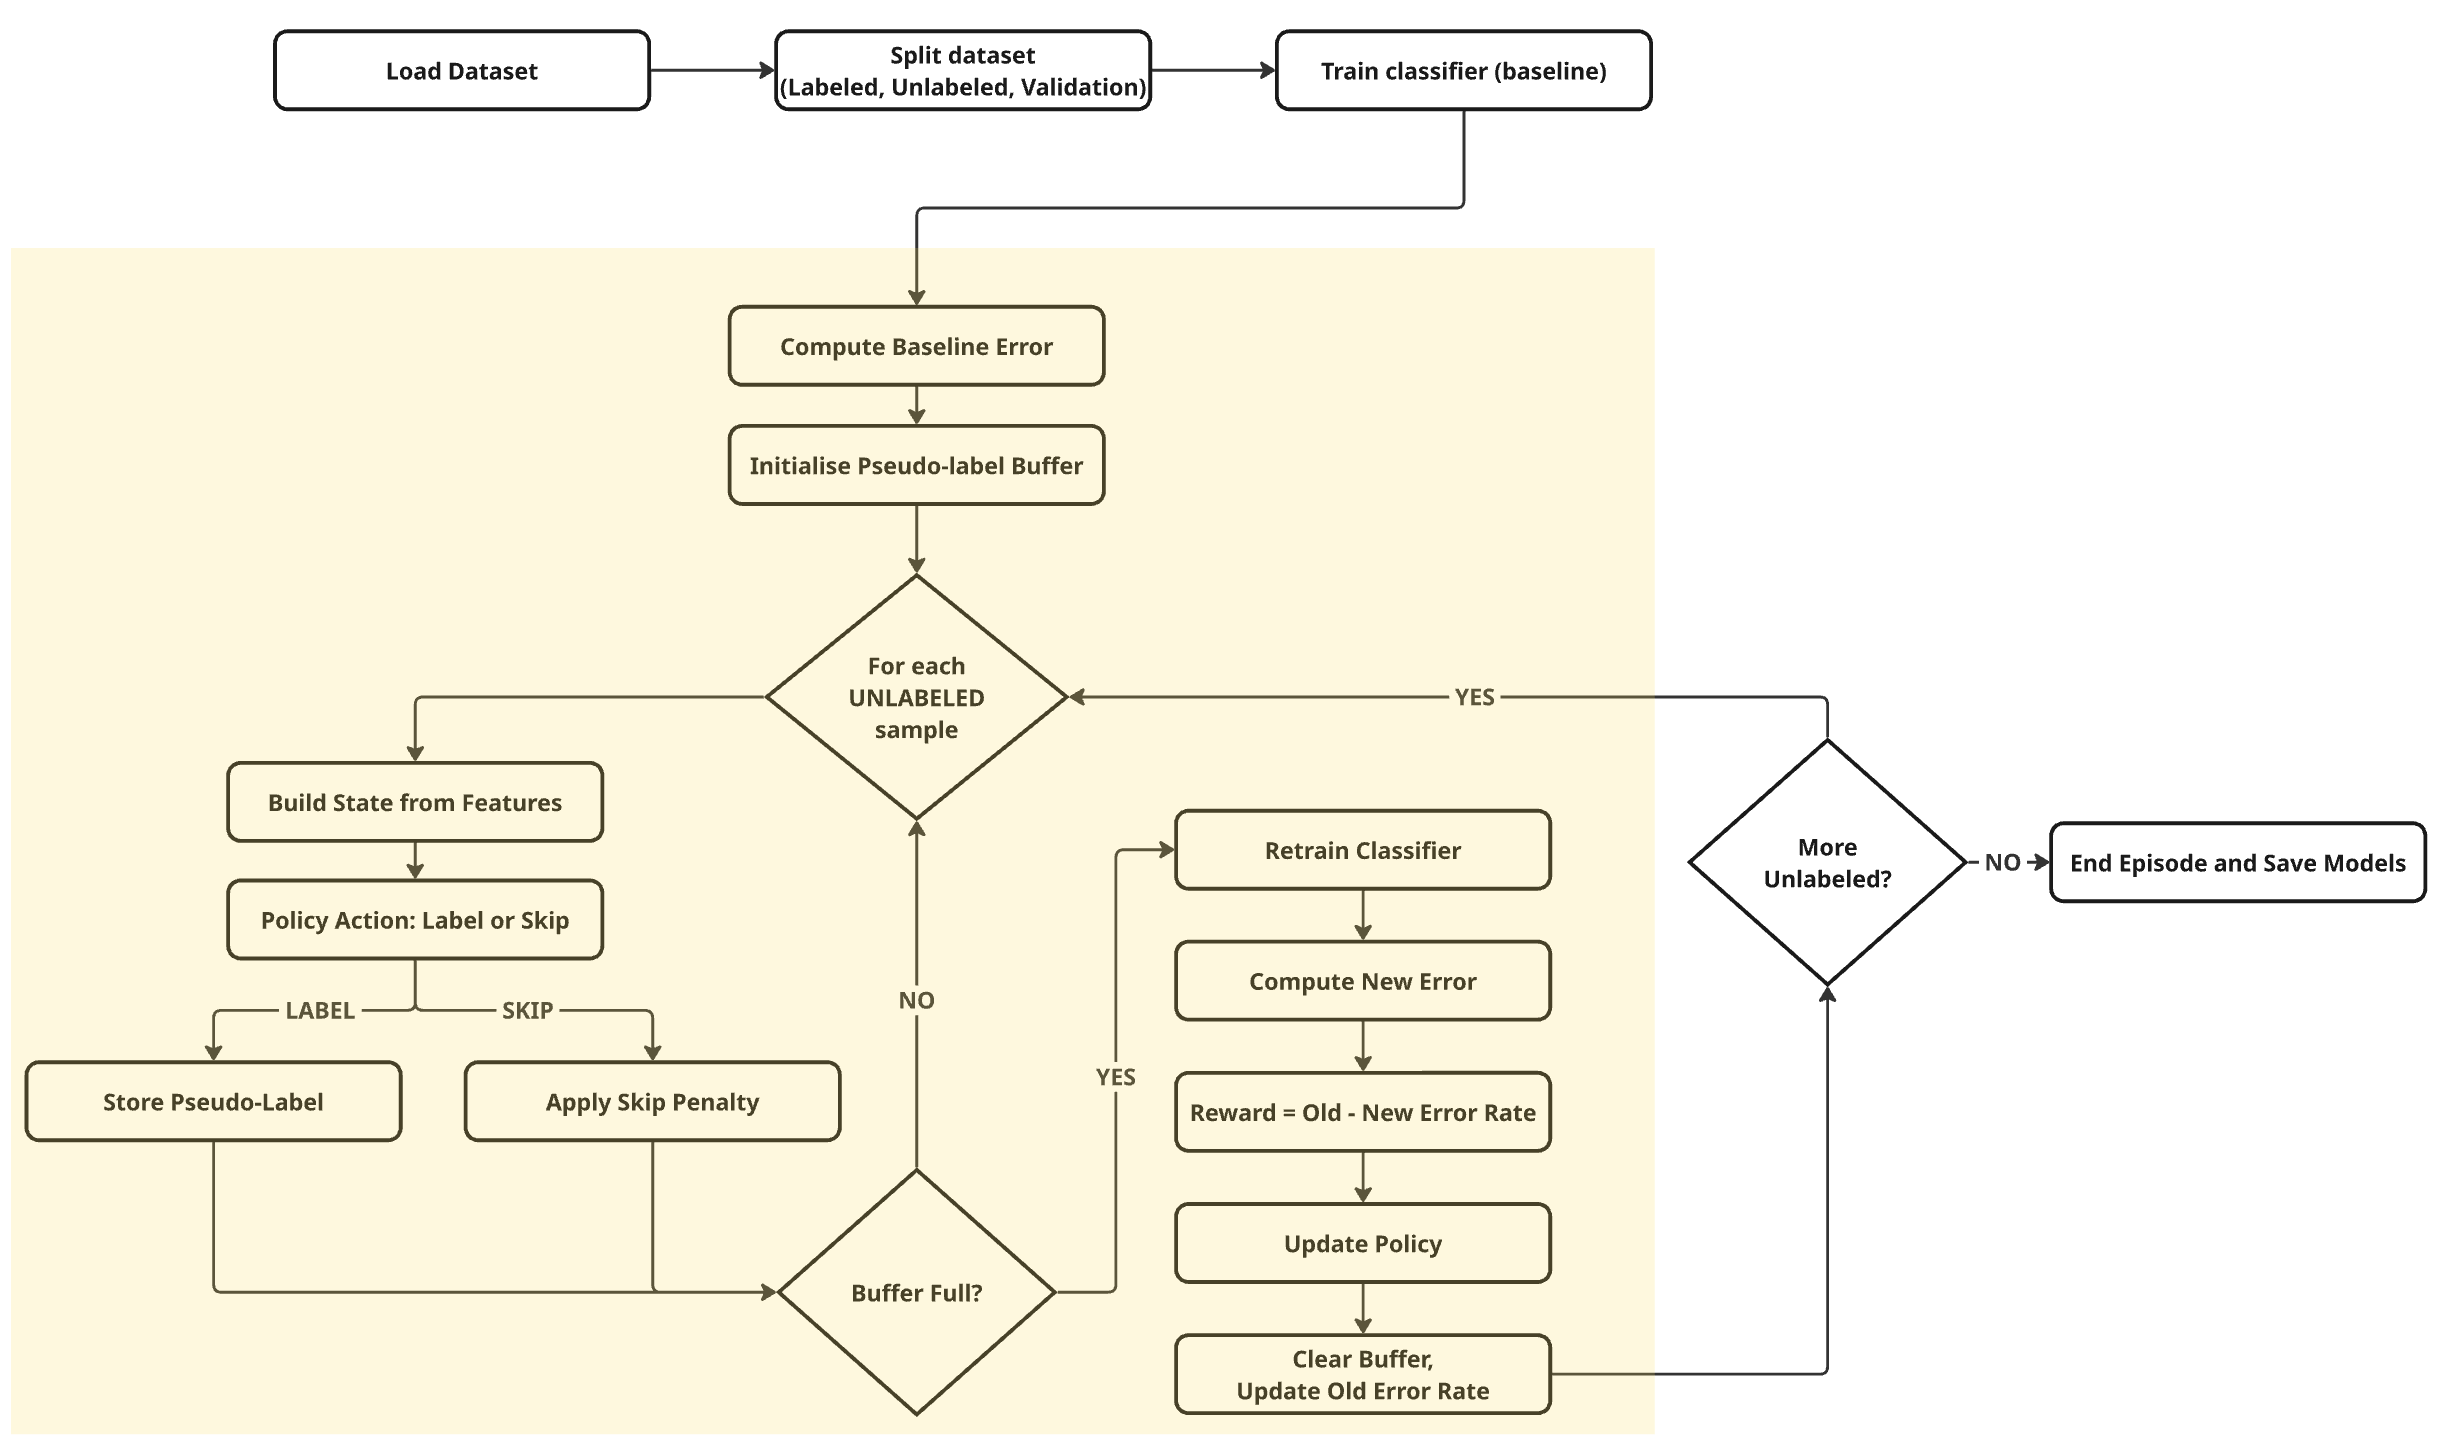
\includegraphics[width=1.0\linewidth]{fig/Flow_Diagram.png} \\


\textbf{State Space ($\mathcal{S}$):} For each unlabeled sample $x_i$, the state $s_i$ is constructed as:
\begin{equation}
s_i = [\phi(x_i), P_\theta(x_i), H(P_\theta(x_i))]
\end{equation}
where:
\begin{itemize}
    \item $\phi(x_i) \in \mathbb{R}^{784}$ are the high level image features derived by passing raw image to the downstream model
    \item $P_\theta(x_i) \in \mathbb{R}^{10}$ are the softmax class probabilities from the downstream model
    \item $H(P_\theta(x_i)) = -\sum_k P_\theta(x_i)_k \log P_\theta(x_i)_k$ is the prediction entropy
\end{itemize}

This representation combines image features, model confidence, and uncertainty, providing the agent with comprehensive information for decision-making.

\textbf{Action Space ($\mathcal{A}$):} The action space consists of $|\mathcal{A}| = K + 1$ discrete actions for a $K$-class classification problem:
\begin{equation}
\mathcal{A} = \{0, 1, \ldots, K-1, \text{skip}\}
\end{equation}
Actions $0$ through $K-1$ assign the corresponding class label as a pseudo-label, while the skip action ($a = K$) indicates the sample should not be pseudo-labeled.

\textbf{Reward Function ($R$):} We designed a confidence-weighted reward function:
\begin{equation}
R(s_i, a_i) = \begin{cases}
-0.1 & \text{if } a_i = \text{skip} \\
P_\theta(x_i)_{a_i} & \text{if } a_i = y_i^{\text{true}} \\
-P_\theta(x_i)_{a_i} & \text{if } a_i \neq y_i^{\text{true}}
\end{cases}
\end{equation}
where $y_i^{\text{true}}$ is the true label (used only for reward computation during training). This design encourages correct, high-confidence predictions while penalizing incorrect ones proportionally to the model's misplaced confidence.

\textbf{Episode Structure:} Each episode processes all $N$ unlabeled samples sequentially. Reward is the absolute difference between the downstream model's error rate for current and the previous batch.
\begin{equation}
R_{\text{final}} = \text{Error}_{\text{new}} - \text{Error}_{\text{old}}
\end{equation}
This provides a delayed reward signal based on the cumulative impact of pseudo-labeling decisions.

\begin{figure}[H]
    \centering
    \includegraphics[width=0.9\textwidth]{fig/flowchart.jpeg}
    \caption{Environment flowchart: reset $\rightarrow$ get state $\rightarrow$ agent action $\rightarrow$ step $\rightarrow$ reward $\rightarrow$ repeat until terminated.}
    \label{fig:env_flowchart}
\end{figure}

\subsubsection{Policy Gradient Agent}

We implemented an Actor-Critic Policy Gradient agent with the following architecture:

\textbf{Policy Network (Actor):} Maps states to action logits:
\begin{align}
h_1 &= \tanh(W_1 s + b_1) \\
h_2 &= \tanh(W_2 h_1 + b_2) \\
\text{logits} &= W_3 h_2 + b_3
\end{align}
where hidden dimensions are 64 neurons per layer.

\textbf{Value Network (Critic):} Estimates state values $V(s)$ using a similar architecture but with scalar output.

\textbf{Training Procedure:} At the end of each episode, we compute:
\begin{itemize}
    \item Rewards-to-go: $G_t = \sum_{t'=t}^T \gamma^{t'-t} r_{t'}$
    \item Advantage estimates: $A_t = G_t - V(s_t)$
    \item Policy loss: $\mathcal{L}_\pi = -\mathbb{E}_t[\log \pi_\theta(a_t|s_t) A_t]$
    \item Value loss: $\mathcal{L}_V = \mathbb{E}_t[(G_t - V(s_t))^2]$
\end{itemize}

Updates are performed using Adam optimizers with learning rates $\alpha_\pi = 10^{-3}$ and $\alpha_V = 10^{-3}$.

\subsubsection{Downstream Model}

The downstream classification model is a Convolutional Neural Network. The specific architecture and parameter counts are detailed in Table~\ref{tab:downstream_architecture} in Section~\ref{sec:results}.

This model is trained on MNIST with cross-entropy loss and serves dual purposes:
\begin{enumerate}
    \item Generating softmax predictions and entropy for state construction
    \item Being the ultimate evaluation metric (validation error rate after pseudo-labeling)
\end{enumerate}

\subsection{Approach 2: RLGSSL Framework}

Inspired by Heidari et al.~\cite{heidari2024rlgssl}, we implemented a complete RLGSSL pipeline with novel adaptive enhancements.

\subsubsection{Teacher-Student Framework}

\begin{figure}[H]
    \centering
    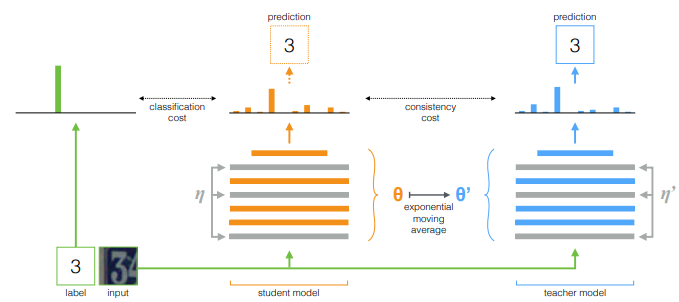
\includegraphics[width=0.9\textwidth]{fig/Student-Teacher Flow.png}
    \caption{ The Mean Teacher method \cite{tarvainen2017mean}. The figure depicts a training batch with a single labeled
    example. Both the student and the teacher model evaluate the input applying noise (η, η0
    ) within
    their computation. The softmax output of the student model is compared with the one-hot label
    using classification cost and with the teacher output using consistency cost. After the weights of the
    student model have been updated with gradient descent, the teacher model weights are updated as an
    exponential moving average of the student weights. Both model outputs can be used for prediction,
    but at the end of the training the teacher prediction is more likely to be correct. A training step with
    an unlabeled example would be similar, except no classification cost would be applied.}
    \label{fig:env_flowchart}
\end{figure}

The teacher model $\theta_T$ maintains an exponential moving average (EMA) of the student model $\theta_S$:
\begin{equation}
\theta_T \leftarrow \beta \theta_T + (1 - \beta) \theta_S
\end{equation}
with decay parameter $\beta = 0.999$. The teacher provides stable pseudo-labels $\tilde{y}_i^u = P_{\theta_T}(x_i^u)$ for unlabeled samples.

\subsubsection{Mixup Data Generation}

For each unlabeled sample $x_i^u$ with teacher pseudo-label $\tilde{y}_i^u$, we sample a labeled example $(x_j^l, y_j^l)$ and create a synthetic mixup sample:
\begin{align}
\mu &\sim \text{Beta}(1.0, 1.0) \\
x_i^m &= \mu x_i^u + (1-\mu) x_j^l \\
y_i^m &= \mu \tilde{y}_i^u + (1-\mu) \text{one-hot}(y_j^l)
\end{align}

This generates continuous interpolations in both feature and label spaces, with $\mu$ determining the mixing ratio.

\subsubsection{RL Reward Function}

The reward signal evaluates how well the student model performs on mixup data:
\begin{equation}
R(s, a; \text{sg}[\theta]) = -\text{MSE}(P_\theta(x_i^m), y_i^m)
\end{equation}
where $\text{sg}[\cdot]$ denotes stop-gradient operation to prevent direct gradient flow through the model parameters during reward computation.

\textbf{Adaptive Enhancements:} We extend the base reward with:
\begin{align}
R_{\text{adaptive}} = R_{\text{base}} &+ \lambda_{\text{conf}} \cdot \mathbb{E}[P_\theta(x_i^m)_{\max} \cdot y_i^m] \\
&+ \lambda_{\text{div}} \cdot H(\mathbb{E}_{\text{batch}}[P_\theta(x^m)]) \\
&+ \lambda_{\text{mix}} \cdot \text{Acc}_{\text{mixup}} \cdot (1 + \sigma(\mu))
\end{align}
where:
\begin{itemize}
    \item Confidence bonus ($\lambda_{\text{conf}} = 0.1$) rewards high-confidence predictions on high-confidence targets
    \item Diversity bonus ($\lambda_{\text{div}} = 0.05$) encourages diverse predictions across the batch
    \item Mixup effectiveness bonus weights performance by $\mu$ diversity
\end{itemize}

\subsubsection{RL Loss Function}

The RL loss combines KL divergence weighting with reward scaling:
\begin{equation}
\mathcal{L}_{\text{rl}} = -\mathbb{E}_{y_i^u \sim \pi_\theta} [\text{KL}(e, y_i^u) \times R(s,a;\text{sg}[\theta])]
\end{equation}
where $e$ is a uniform baseline distribution over classes.

\textbf{Adaptive Enhancements:}
\begin{itemize}
    \item \textbf{Curriculum Learning}: Gradually increase focus on high-confidence samples:
    \begin{equation}
    w_{\text{curriculum}} = \min\left(1.0, \frac{\text{epoch}}{\text{max\_epochs} \times 0.5}\right)
    \end{equation}
    
    \item \textbf{Entropy Regularization}: Prevent overconfident predictions:
    \begin{equation}
    \mathcal{L}_{\text{rl}}^{\text{adaptive}} = \mathcal{L}_{\text{rl}} + \lambda_{\text{entropy}} H(\tilde{y}_i^u)
    \end{equation}
    with $\lambda_{\text{entropy}} = 0.01$
    
    \item \textbf{Confidence-Based Weighting}: Focus learning on reliable pseudo-labels:
    \begin{equation}
    w_i = \mathbb{1}[\max(\tilde{y}_i^u) > \tau] \cdot (1 + w_{\text{curriculum}})
    \end{equation}
    with threshold $\tau = 0.8$
\end{itemize}

\subsubsection{Combined Loss Function}

The total training loss integrates supervised, consistency, and RL components:
\begin{equation}
\mathcal{L}_{\text{total}} = \mathcal{L}_{\text{sup}} + \lambda_{\text{cons}} \mathcal{L}_{\text{cons}} + \lambda_{\text{rl}} \mathcal{L}_{\text{rl}}^{\text{adaptive}}
\end{equation}
where:
\begin{itemize}
    \item $\mathcal{L}_{\text{sup}} = \text{CrossEntropy}(P_\theta(x^l), y^l)$ on labeled data
    \item $\mathcal{L}_{\text{cons}} = \text{MSE}(P_\theta(x^u), P_{\theta_T}(x^u))$ enforces student-teacher consistency
    \item Default weights: $\lambda_{\text{cons}} = 0.1$, $\lambda_{\text{rl}} = 0.1$
\end{itemize}

\subsection{Implementation Details}

\textbf{Framework:} PyTorch 2.0 with CUDA support

\textbf{Datasets:}
\begin{itemize}
    \item Policy Gradient approach: MNIST (18000 labeled, 40000 unlabeled, 2000 validation)
    \item RLGSSL approach: CIFAR-10 (1000/2000/4000 labeled settings)
\end{itemize}

\textbf{Training Configuration:} Detailed hyperparameter configurations for both the Policy Gradient and RLGSSL approaches (including learning rates, batch sizes, and decay parameters) are provided in Table~\ref{tab:hyperparameters} in Section~\ref{sec:results}.

\textbf{Computational Environment:} Device: GPU, VRAM: 16GB

\textbf{Code Repository:} \url{https://github.com/phanindra-max/fall-2025-group11}

% ------------------------------------------------------------------------------------------------------------------------

\section{Results and Discussion}
\label{sec:results}

This section presents our experimental results, including training dynamics, performance metrics, and analysis of the challenges encountered during implementation.

\subsection{Experimental Setup}

\subsubsection{Dataset Configuration}

\textbf{Policy Gradient Experiments (MNIST):}
\begin{itemize}
    \item Total Training Samples: 60,000
    \item Labeled Samples: 18,000
    \item Unlabeled Samples: 40,000
    \item Validation Samples: 2,000
    \item Test Samples: 10,000
\end{itemize}

\textbf{RLGSSL Experiments (CIFAR-10):}
\begin{itemize}
    \item Total Training Samples: 50,000
    \item Labeled Samples: 1000/2000/4000 (2\%/4\%/8\%)
    \item Unlabeled Samples: 49,000/48,000/46,000
    \item Test Samples: 10,000
\end{itemize}

\subsubsection{Model Architectures}

\textbf{Policy Gradient Downstream Model:}
\begin{table}[H]
    \centering
    \begin{tabular}{lrr}
        \hline
        \textbf{Layer} & \textbf{Output Shape} & \textbf{Parameters} \\
        \hline
        Conv2D (1→32, 3×3, padding=1) & 32×28×28 & 320 \\
        MaxPool2D (2×2) & 32×14×14 & 0 \\
        Conv2D (32→64, 3×3, padding=1) & 64×14×14 & 18,496 \\
        MaxPool2D (2×2) & 64×7×7 & 0 \\
        Conv2D (64→128, 3×3, padding=1) & 128×7×7 & 73,856 \\
        AdaptiveAvgPool2D (1×1) & 128×1×1 & 0 \\
        FC (128→10) & 10 & 1,290 \\
        \hline
        \textbf{Total} & & \textbf{93,962} \\
        \hline
    \end{tabular}
    \caption{Updated architecture of the downstream CNN model for MNIST classification}
    \label{tab:downstream_architecture}
\end{table}


\textbf{RLGSSL Model:}
\begin{itemize}
    \item Architecture: CNN-13
    \begin{itemize}
        \item \textbf{Block 1}
        \begin{itemize}
            \item Conv1: $3 \rightarrow 128$, $3{\times}3$, padding 1
            \item BatchNorm
            \item Conv2: $128 \rightarrow 128$, $3{\times}3$, padding 1
            \item BatchNorm
            \item Conv3: $128 \rightarrow 128$, $3{\times}3$, padding 1
            \item BatchNorm
            \item MaxPool $2{\times}2$
            \item Dropout $p=0.25$
        \end{itemize}

        \item \textbf{Block 2}
        \begin{itemize}
            \item Conv4: $128 \rightarrow 256$, $3{\times}3$, padding 1
            \item BatchNorm
            \item Conv5: $256 \rightarrow 256$, $3{\times}3$, padding 1
            \item BatchNorm
            \item Conv6: $256 \rightarrow 256$, $3{\times}3$, padding 1
            \item BatchNorm
            \item MaxPool $2{\times}2$
            \item Dropout $p=0.25$
        \end{itemize}

        \item \textbf{Block 3}
        \begin{itemize}
            \item Conv7: $256 \rightarrow 512$, $3{\times}3$, \textbf{no padding}
            \item BatchNorm
            \item Conv8: $512 \rightarrow 256$, $1{\times}1$
            \item BatchNorm
            \item Conv9: $256 \rightarrow 128$, $1{\times}1$
            \item BatchNorm
        \end{itemize}

        \item \textbf{Additional Convolution Layers}
        \begin{itemize}
            \item Conv10: $128 \rightarrow 128$, $3{\times}3$, padding 1
            \item BatchNorm
            \item Conv11: $128 \rightarrow 128$, $3{\times}3$, padding 1
            \item BatchNorm
            \item Conv12: $128 \rightarrow 128$, $3{\times}3$, padding 1
            \item BatchNorm
        \end{itemize}

        \item \textbf{Final Layers}
        \begin{itemize}
            \item AdaptiveAvgPool: output $1\times1$
            \item Dropout $p=0.5$
            \item Fully Connected: $128 \rightarrow \text{num\_classes}$
        \end{itemize}
    \end{itemize}

    \item Total Parameters: 3,567,370
    \item Trainable Parameters: 3,567,370
\end{itemize}


\subsubsection{Hyperparameters}

\begin{table}[H]
    \centering
    \begin{tabular}{lcc}
        \hline
        \textbf{Parameter} & \textbf{Policy Gradient} & \textbf{RLGSSL} \\
        \hline
        Learning Rate & $10^{-3}$ & $10^{-3}$ \\
        Batch Size & 256 & 128 \\
        Episodes/Epochs & 50 & 50+400 \\
        Discount Factor ($\gamma$) & 0.99 & N/A \\
        EMA Decay ($\beta$) & N/A & 0.999 \\
        Mixup Alpha ($\alpha$) & N/A & 1.0 \\
        $\lambda_{\text{sup}}$ & N/A & 0.1 \\
        $\lambda_{\text{cons}}$ & N/A & 0.1 \\
        $\lambda_{\text{rl}}$ & N/A & 0.1 \\
        Confidence Threshold & N/A & 0.8 \\
        Confidence Weight & N/A & 0.1 \\
        Diversity Weight & N/A & 0.05 \\
        Entropy Regularization & N/A & 0.01 \\
        \hline
    \end{tabular}
    \caption{Hyperparameter configurations for both approaches}
    \label{tab:hyperparameters}
\end{table}

\subsection{Policy Gradient Results}
\begin{table}[h]
\centering
\begin{tabular}{lcc}
\hline
\textbf{} & \textbf{MNIST} & \textbf{CIFAR-10} \\
\hline
cnn      & 3.45\%  & 34.40\% \\
mlp      & 37.40\% & 59.60\% \\
resnet18 & 5.80\%  & 25.75\% \\
\hline
\end{tabular}
\caption{Performance comparison on MNIST and CIFAR-10}
\end{table}

\textbf{Key Observations:}
\begin{itemize}
    \item Initial baseline error rate: $\sim$54\%
    \item Final best error rate: $\sim$3.45\%
\end{itemize}

\subsection{RLGSSL Results}

\subsubsection{Training Progression}

Table~\ref{tab:rlgssl_training} shows the training dynamics observed during RLGSSL experiments on CIFAR-10 with 1000 labeled samples.

\begin{table}[H]
    \centering
    \begin{tabular}{cccccl}
        \hline
        \textbf{Epoch} & \textbf{Error (\%)} & \textbf{Loss} & \textbf{RL Loss} & \textbf{Reward} & \textbf{Notes} \\
        \hline
        50 (warmup) & 53.61 & 0.137 & -0.00533 & -0.0305168 & Stable supervised learning but weak teacher. \\
        100 & 74.02 & 0.233 & 0.018 & -0.0298085 & Error increases as RL is introduced. \\
        150 & 66.56 & 0.215 & 0.013 & -0.029022 & Partial recovery; RL signals still unstable. \\
        250 & 59.48 & 0.188 & 0.005 & -0.0290487 & Training stabilizes; gradual improvement. \\
        350 & 61.51 & 0.1601 & -0.00464 & -0.0283258 & Mild fluctuations. \\
        450 & 58.59 & 0.13346 & -0.03042 & -0.0281552 & Converging slowly. \\
        \hline
    \end{tabular}
    \caption{RLGSSL training progression on CIFAR-10 (1000 labels).}
    \label{tab:rlgssl_training}
\end{table}



\textbf{Performance Metrics:}
\begin{itemize}
    \item \textbf{Best Student Error Rate:} 53.8\%
    \item \textbf{Training Time:} $\sim$10 hours
\end{itemize}

\subsubsection{Comparison with Literature}

\textbf{Analysis Gap:} Our best observed error rate of 53.8\% is significantly below the paper's reported 9.15\% error. This discrepancy likely stems from:
\begin{itemize}
    \item Potential bugs in adaptive enhancement implementations
    \item Need for more careful hyperparameter tuning
    \item Possible differences in data preprocessing or augmentation strategies
\end{itemize}


% ------------------------------------------------------------------------------------------------------------------------

\section{Discussion}

This section reflects on the key challenges encountered, lessons learned, and insights gained throughout the project implementation.

\subsection{Overview of Findings}
Our experiments highlighted distinct trade-offs between the two approaches. The \textbf{Policy Gradient agent} demonstrated adaptive behavior, successfully learning to balance pseudo-labeling with skipping uncertain samples. Conversely, the \textbf{RLGSSL framework} showed promise with stable training.

Despite successfully implementing the full pipelines, we observed significant performance gaps compared to state-of-the-art benchmarks. These gaps were primarily driven by computational constraints preventing full convergence and numerical instabilities in our adaptive reward enhancements.

\subsection{Technical Challenges}
% ... Continue with your existing text regarding Reward Function Design ...

\subsubsection{Reward Function Design}

Designing effective reward functions proved to be one of the most challenging aspects. Sparse vs. dense rewards presented an issue: initial experiments with only end-of-episode error rate rewards provided insufficient learning signal, and adding per-step confidence-based rewards improved learning but introduced new challenges. Reward scaling was also difficult, as balancing the magnitude of step rewards (confidence values in [0,1]) with episode-end error rate bonuses (potentially large) required careful tuning. Stability issues emerged because the adaptive reward enhancements in RLGSSL introduced numerical instability; the diversity bonus, in particular, may have caused gradient explosions when batch entropy varied significantly.

\textbf{Recommendation:} Future work should implement reward clipping and normalization strategies used in modern RL algorithms like PPO.

\subsubsection{Computational Constraints}

The computational demands of RL-based pseudo-labeling present significant practical barriers. Episode length was a concern because each Policy Gradient episode processes all 4000 unlabeled samples, resulting in lengthy episodes and delayed learning. CPU limitations were evident as training on CPU for 15+ hours without completion highlights the need for GPU acceleration; however, even with GPUs, the approach may struggle to scale to ImageNet-scale datasets. Memory requirements also posed challenges, as maintaining teacher and student models simultaneously, along with mixup sample generation, doubles memory requirements compared to standard training.

\textbf{Recommendation:} Investigate mini-batch RL approaches and gradient accumulation strategies to improve computational efficiency.

\subsubsection{Non-Stationarity and Credit Assignment}

The pseudo-labeling environment violates key RL assumptions. The moving target issue arises because the downstream model evolves during training, causing state distributions to shift continuously and challenging standard RL convergence guarantees. Delayed feedback complicates training because error rate improvements may not manifest until many episodes later, making credit assignment difficult and raising the question of which pseudo-labels at which training iterations contributed to final performance. Exploration–exploitation adds further complexity, as balancing exploration of uncertain samples versus exploitation of confident predictions is complicated by the fact that exploration today affects future model capabilities.

\textbf{Recommendation:} Consider meta-learning approaches where the policy is trained across multiple dataset/model combinations to develop more robust pseudo-labeling strategies.

\subsection{Insights on RLGSSL Formulation}

Through implementation, we gained several insights into the RLGSSL approach.

\subsubsection{Policy Network as Classifier}

The elegant formulation where the classifier itself serves as the RL policy eliminates architectural complexity but introduces subtleties. Gradient flow must be handled carefully, and careful use of stop-gradient operations is crucial to prevent the model from “hacking” rewards by simply memorizing mixup samples. Loss weighting is also critical; the relative weights of supervised, consistency, and RL losses dramatically affect behavior, and in our experiments, RL loss dominated when set too high, causing instability. Curriculum necessity becomes clear as the curriculum learning component is not just an enhancement but appears necessary for stability, gradually introducing RL objectives as the model matures.

\subsubsection{Mixup as Environment Dynamics}

Using mixup to create the “environment” for RL is creative but has implications. Sample efficiency benefits from mixup because it provides infinite synthetic samples, enabling dense RL learning signals. Smoothness is enhanced as continuous interpolation in mixup may help smooth the reward landscape, potentially aiding RL optimization. Generalization may improve from training on mixup samples through better interpolation behavior, though extrapolation (out-of-distribution samples) remains challenging.

\subsection{Comparison: Policy Gradient vs. RLGSSL}

Table~\ref{tab:approach_comparison} compares the two approaches implemented.

\begin{table}[H]
    \centering
    \begin{tabular}{p{3cm}p{5cm}p{5cm}}
        \hline
        \textbf{Aspect} & \textbf{Policy Gradient} & \textbf{RLGSSL} \\
        \hline
        Complexity & Higher: separate RL agent + downstream model & Lower: unified architecture \\
        Scalability & Poor: full episode required & Better: mini-batch training \\
        Interpretability & Higher: explicit state-action mapping & Lower: implicit RL in loss function \\
        Flexibility & Higher: easy to modify reward/state & Lower: coupled to mixup strategy \\
        Performance & Moderate: Sensitive to reward shaping and batching implementation & Higher: Computationally expensive because of complex architectures. \\
        Stability & Lower: Less stable because of sparse rewards & Moderate: Issues with adaptive enhancements, but better stability with Teacher Student framework \\
        \hline
    \end{tabular}
    \caption{Comparison of the two RL-based pseudo-labeling approaches}
    \label{tab:approach_comparison}
\end{table}

\subsection{Practical Considerations}

\subsubsection{When to Use RL for Pseudo-Labeling}

Based on our experience, RL-based pseudo-labeling is most appropriate when labeled data is extremely limited ($<$1\% of dataset), pseudo-labeling decisions have long-term consequences (e.g., medical diagnosis), computational resources are available for extensive training, and the problem exhibits clear reward signals (e.g., validation error rate).

It may be overkill when labeled data is moderately available ($>$10\% of dataset), simple confidence thresholding already works well, real-time or resource-constrained deployment is required, or the dataset is extremely large (millions of samples).

\subsubsection{Engineering Recommendations}

From an engineering perspective, several practices proved valuable. Modular design, where environment, agent, and downstream model are separated into distinct modules, facilitated debugging and experimentation. Logging infrastructure, particularly comprehensive logging with TensorBoard, was essential for diagnosing training dynamics and stability issues. Checkpointing provided reliability, as regular model checkpointing allowed recovery from crashes and comparison of models at different training stages. Ablation-friendly code supported rapid experimentation, as designing hyperparameters and enhancement flags in a central config file enabled rapid ablation studies.

\subsection{Limitations of Current Work}

We acknowledge several limitations. Limited datasets were used, as experiments focused on MNIST and CIFAR-10; generalization to other domains (text, speech, medical imaging) remains unexplored. Hyperparameter sensitivity remains a concern since the limited computational budget prevented extensive hyperparameter searches. Comparison baselines are missing because direct comparisons with strong SSL baselines like FixMatch, MixMatch, or simple confidence thresholding were not performed. Theoretical analysis is another limitation, as no formal convergence guarantees or theoretical characterization of when RL-based pseudo-labeling should outperform alternatives were provided.


% ------------------------------------------------------------------------------------------------------------------------

\section{Conclusion}

This capstone project investigated the application of reinforcement learning to intelligent pseudo-labeling in semi-supervised learning contexts. We developed and evaluated two complementary approaches: a custom Policy Gradient framework with explicit state-action formulations, and an implementation of the novel RLGSSL approach with adaptive enhancements.

\subsection{Key Contributions}

Our work makes several contributions:

\begin{enumerate}
    \item \textbf{Complete RL Framework:} Developed a full-featured custom OpenAI Gymnasium environment for pseudo-labeling, including carefully designed state spaces (image features + model predictions + entropy), action spaces (label assignment or skip), and confidence-weighted reward functions.
    
    \item \textbf{RLGSSL Implementation:} Successfully implemented the RLGSSL framework proposed by Heidari et al., including teacher-student architecture, mixup augmentation, and the novel RL reward formulation.
    
    \item \textbf{Adaptive Enhancements:} Extended RLGSSL with confidence bonuses, diversity regularization, curriculum learning, and entropy regularization mechanisms not present in the original paper.
    
    \item \textbf{Practical Insights:} Documented computational challenges, stability issues, and engineering considerations crucial for practitioners attempting to apply RL to pseudo-labeling.
    
    \item \textbf{Open-Source Implementation:} Provided well-documented, modular code for future research and experimentation.
\end{enumerate}

\subsection{Main Findings}

\textbf{Technical Feasibility:} RL-based pseudo-labeling is technically feasible and can be implemented using standard deep RL techniques. However, significant engineering effort is required to achieve stability and scalability.

\textbf{Computational Demands:} Both approaches exhibit substantial computational requirements, with training times exceeding 15 hours on CPU for moderate-scale experiments. GPU acceleration and algorithmic optimizations are essential for practical deployment.

\textbf{Stability Challenges:} Adaptive reward enhancements, while theoretically motivated, introduced numerical instability. Careful implementation with gradient clipping and reward normalization is crucial.

\textbf{Performance Gap:} Our results showed a significant gap compared to state-of-the-art SSL methods, likely due to incomplete training, implementation bugs, and insufficient hyperparameter tuning. This highlights the challenge of reproducing research results and the importance of careful validation.

\subsection{Lessons Learned}

\textbf{Reward Engineering is Critical:} The choice and design of reward functions dramatically affects learning dynamics. Simple confidence-based rewards worked reasonably well, but complex multi-component rewards require careful balancing and stability mechanisms.

\textbf{Start Simple, Add Complexity Gradually:} Our experience suggests starting with minimal RL formulations and incrementally adding enhancements while rigorously testing stability at each stage.

\textbf{Computational Planning is Essential:} RL-based approaches require significantly more computation than standard SSL. Projects should budget computational resources accordingly and prioritize access to GPU infrastructure.

\textbf{Reproducibility is Challenging:} Even with detailed papers, reproducing research results requires careful attention to implementation details, data preprocessing, and hyperparameter settings that may not be fully documented.

\subsection{Broader Impact}

This work contributes to the growing body of research applying reinforcement learning to data-centric AI problems. As labeled data remains a bottleneck in many domains—especially in medical imaging, autonomous systems, and low-resource languages—intelligent pseudo-labeling strategies could significantly reduce annotation costs and democratize access to machine learning.

However, practitioners should be aware of the computational costs and implementation complexity. For many applications, simpler SSL baselines (FixMatch, MixMatch) may provide better cost-benefit trade-offs. RL-based approaches are most valuable when:
\begin{itemize}
    \item Labeled data is extremely scarce ($<$1\% of dataset)
    \item Label quality is critical (high-stakes domains)
    \item Computational resources are available
    \item The problem exhibits clear, measurable objectives
\end{itemize}

\subsection{Future Work}
To build upon this foundation, future research should focus on stabilizing training dynamics using PPO-style trust region constraints and gradient normalization. Additionally, conducting comprehensive ablation studies to isolate the impact of curriculum learning and confidence bonuses is essential. Finally, scaling the framework via mini-batch RL methods would allow for validation on larger, more complex datasets beyond CIFAR-10.

\subsection{Closing Remarks}

This capstone project demonstrated both the promise and challenges of applying reinforcement learning to semi-supervised learning. While we encountered significant obstacles—training instability, computational constraints, and performance gaps—the experience provided valuable insights into the complexities of RL-based data-centric AI.

The field of RL-guided semi-supervised learning remains in its early stages, with much room for innovation. As computational resources become more accessible and RL algorithms continue to improve, intelligent pseudo-labeling may become a standard tool in the machine learning practitioner's toolkit.

We hope this work serves as a foundation for future researchers and provides both inspiration and cautionary lessons for those embarking on similar projects.

\bibliographystyle{IEEEtran}
\bibliography{references}


%------ To create Appendix with additional stuff -------%
\newpage
\appendix
\section{Appendix}

\subsection{A: Code Structure}

The project codebase is organized as follows:

\begin{verbatim}
Capstone/
├── src/
│   ├── component/
│   │   ├── main.py           # Main training loop (Policy Gradient)
│   │   ├── model.py          # Policy and Value Networks
│   │   ├── env.py            # Custom PseudoLabelEnv
│   │   ├── utils.py          # Helper functions
│   │   └── config.py         # Hyperparameter configuration
│   └── requirements.txt      # Python dependencies
├── reports/
│   ├── RLGSSL_Report_Draft.md     # RLGSSL implementation notes
│   ├── Progress_Report/
│   │   └── Progress_Report.md     # Weekly progress tracking
│   └── Latex_report/
│       ├── Final_Report.tex       # This document
│       ├── Sample_Report.tex      # Template
│       ├── File_Setup.tex         # LaTeX configuration
│       ├── references.bib         # Bibliography
│       └── fig/                   # Figures directory
└── README.md                      # Project overview
\end{verbatim}

\subsection{B: Hyperparameter Configuration}

Complete hyperparameter settings used in experiments:

\textbf{Policy Gradient (config.py):}
\begin{lstlisting}[language=Python]
# Training parameters
EPISODES = 50
NUM_LABELED = 1000
NUM_UNLABELED = 4000
NUM_VALIDATION = 1000

# Policy Gradient parameters
GAMMA = 0.99
ALPHA_PI = 1e-3
ALPHA_V = 1e-3
HIDDEN_DIM = 64
POLICY_TYPE = 'mlp'

# Downstream Model parameters
DOWNSTREAM_LR = 0.001
DOWNSTREAM_EPOCHS = 1
BATCH_SIZE = 32
\end{lstlisting}

\textbf{RLGSSL (from draft documentation):}
\begin{lstlisting}[language=Python]
# Training Configuration
WARMUP_EPOCHS = 50
RLGSSL_EPOCHS = 400
BATCH_SIZE = 128
LEARNING_RATE = 0.001

# Teacher-Student
EMA_DECAY = 0.999

# Mixup
MIXUP_ALPHA = 1.0

# Loss Weights
LAMBDA_SUP = 1.0
LAMBDA_CONS = 0.1
LAMBDA_RL = 0.1

# Adaptive Enhancements
CONFIDENCE_THRESHOLD = 0.8
CONFIDENCE_WEIGHT = 0.1
DIVERSITY_WEIGHT = 0.05
ENTROPY_REGULARIZATION = 0.01
\end{lstlisting}

\subsection{C: Key Implementation Details}

\textbf{EMA Teacher Update:}
\begin{lstlisting}[language=Python]
def update_ema_teacher(student_model, teacher_model, beta=0.999):
    for teacher_param, student_param in zip(
        teacher_model.parameters(), 
        student_model.parameters()
    ):
        teacher_param.data = (
            beta * teacher_param.data + 
            (1 - beta) * student_param.data
        )
\end{lstlisting}

\textbf{Mixup Generation:}
\begin{lstlisting}[language=Python]
def generate_mixup(unlabeled_batch, labeled_batch, alpha=1.0):
    mu = np.random.beta(alpha, alpha)
    x_u, pseudo_y_u = unlabeled_batch
    x_l, y_l = labeled_batch
    
    # Create mixup samples
    x_m = mu * x_u + (1 - mu) * x_l
    y_m = mu * pseudo_y_u + (1 - mu) * F.one_hot(y_l)
    
    return x_m, y_m, mu
\end{lstlisting}

\textbf{Confidence-Based Reward:}
\begin{lstlisting}[language=Python]
def calculate_reward(pred_label, true_label, action, probs):
    if action == num_classes:  # skip action
        return -0.1
    confidence = probs[action].item()
    if action == true_label:
        return confidence  # positive reward for correct
    else:
        return -confidence  # negative reward for incorrect
\end{lstlisting}

\subsection{D: References for Additional Reading}

\textbf{Reinforcement Learning Fundamentals:}
\begin{itemize}
    \item Sutton \& Barto (2018), ``Reinforcement Learning: An Introduction'' (2nd Edition)
    \item Schulman et al. (2017), ``Proximal Policy Optimization Algorithms''
    \item Mnih et al. (2016), ``Asynchronous Methods for Deep Reinforcement Learning''
\end{itemize}

\textbf{OpenAI Gymnasium:}
\begin{itemize}
    \item Official Documentation: \url{https://gymnasium.farama.org/}
    \item Custom Environment Tutorial: \url{https://gymnasium.farama.org/tutorials/gymnasium_basics/environment_creation/}
\end{itemize}

\end{document}

